\documentclass[../main.tex]{subfiles}

\begin{figure}[ht]
    \centering
    \begin{subfigure}[b]{0.3\textwidth}
        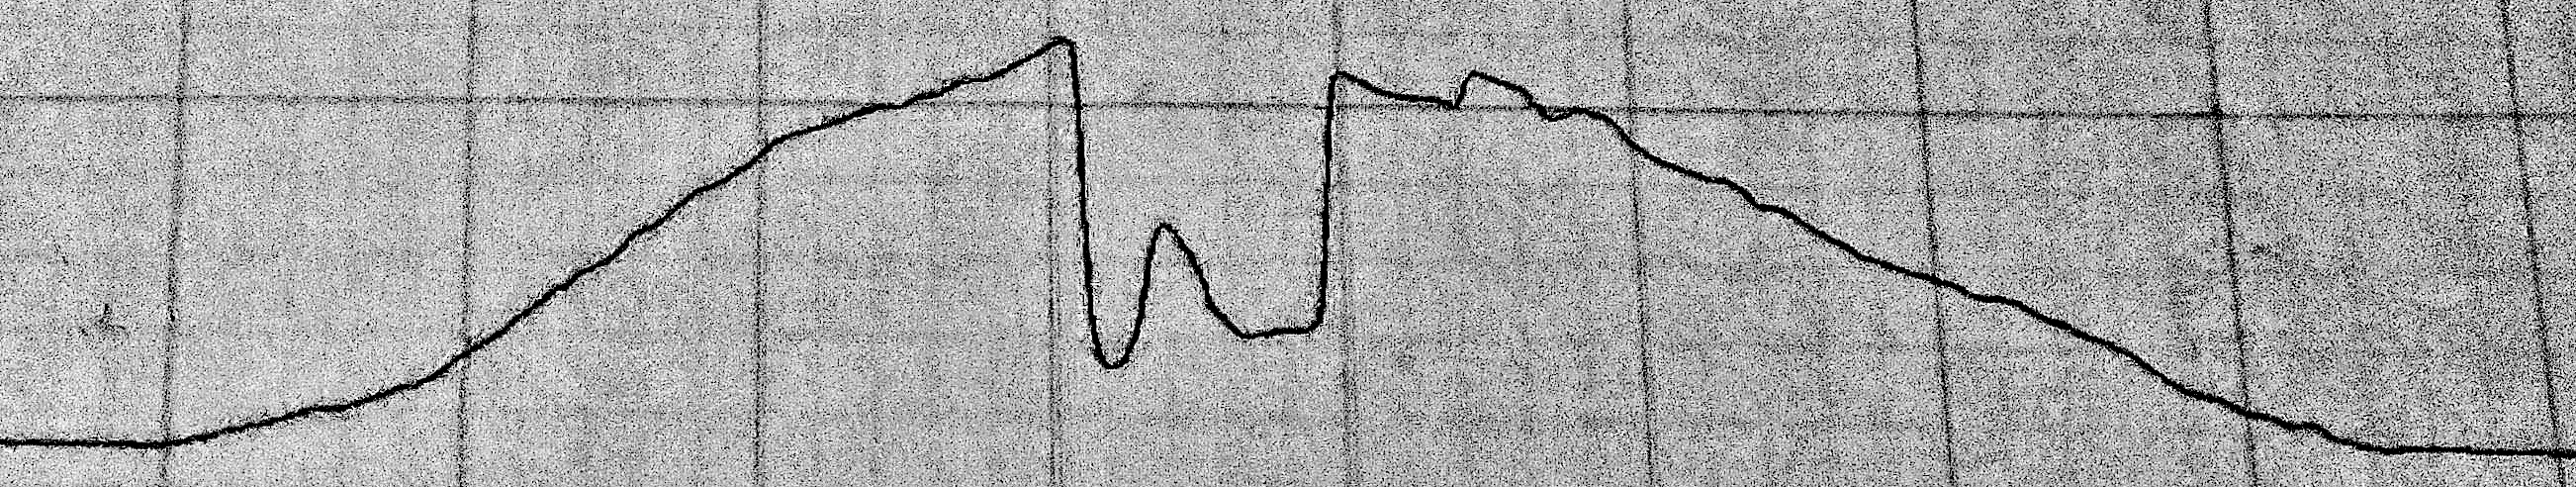
\includegraphics[width=\textwidth]{experiment/spectra/21c-diagramm-600-pro-mm.png}
        \caption{600 Linien / mm}
    \end{subfigure}
    \begin{subfigure}[b]{0.3\textwidth}
        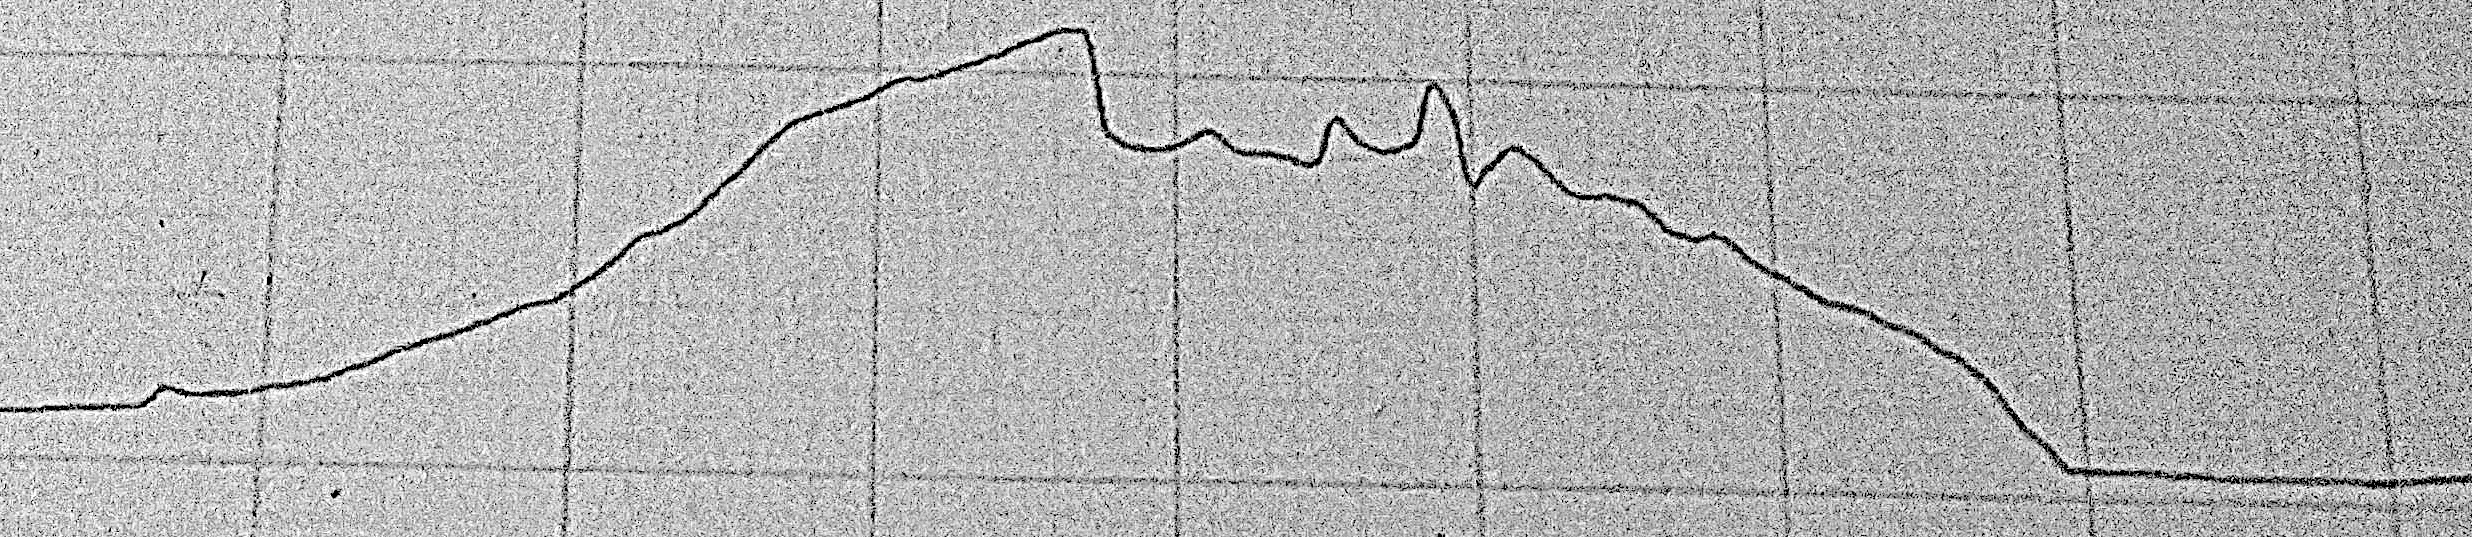
\includegraphics[width=\textwidth]{experiment/spectra/27c-diagramm-leypold.png}
        \caption{Leybold}
    \end{subfigure}
    \begin{subfigure}[b]{0.3\textwidth}
        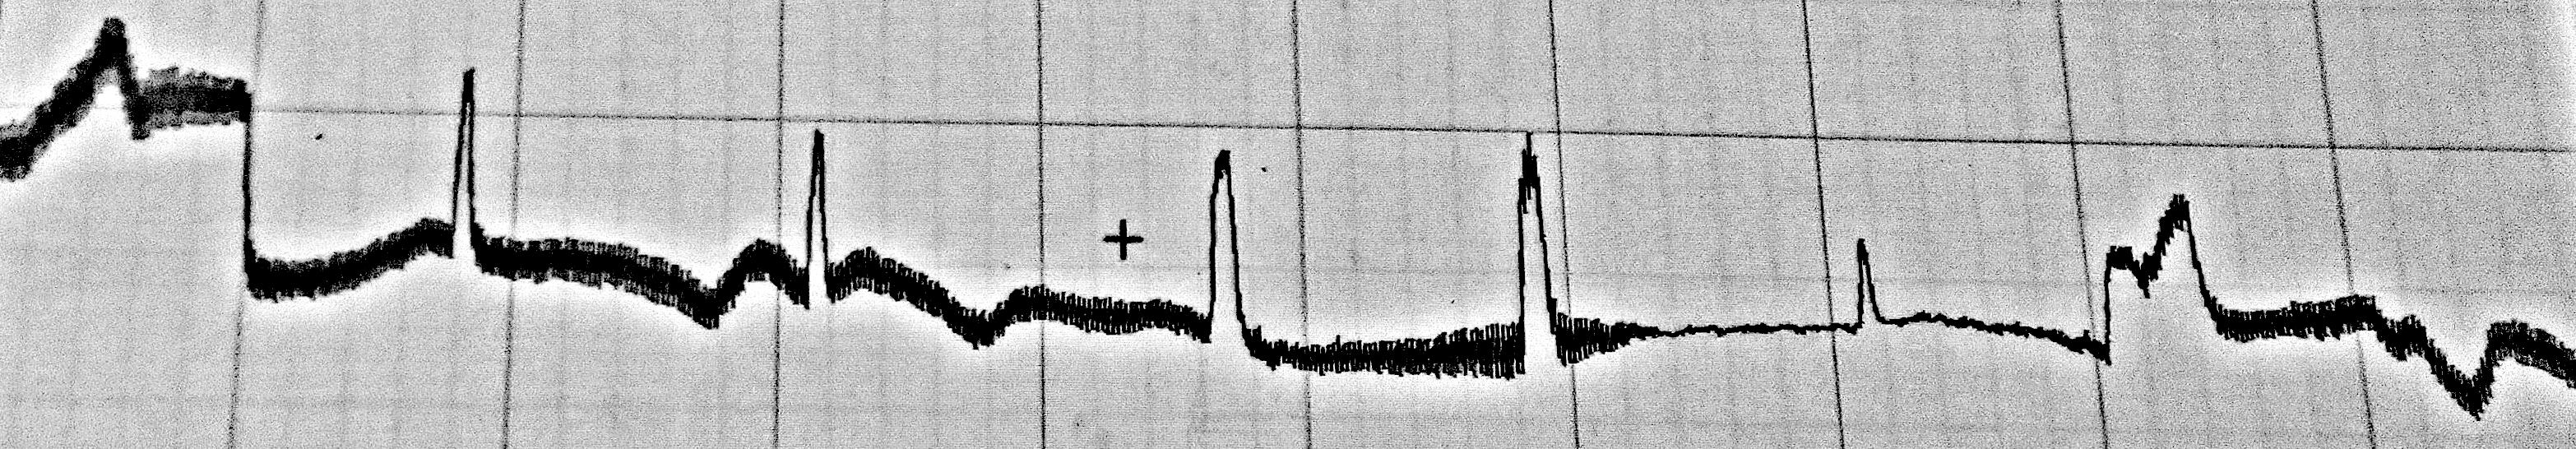
\includegraphics[width=\textwidth]{experiment/spectra/30c-diagramm-reflexionsgitter.png}
        \caption{Reflexionsgitter}
    \end{subfigure}
    \caption{Spektra verschiedener Gitter}
\end{figure}

% Diagramme
% Fehler
